\documentclass{standalone}

\usepackage{tikz}
\usetikzlibrary{calc}

\begin{document}

    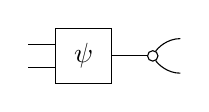
\begin{tikzpicture}[yscale=-1,x=1em,y=1.25em]
        
        \node (J1) [draw, minimum height = 2em, minimum width = 2em, fill=white] at (0,0){$\psi$};
        \coordinate (J1I1) at ($(J1) +(-1,-0.33)$);
        \coordinate (J1I2) at ($(J1) +(-1,0.33)$);
        \coordinate (J1O1) at ($(J1) +(1,0)$);
        \node (C1) [draw, circle, fill=white, scale=0.4] at ($(J1) +(2.5,0)$) {};

        \coordinate (O1) at ($(C1) +(1,-0.5)$);
        \coordinate (O2) at ($(C1) +(1,0.5)$);

        \draw ($(J1I1) +(-1,0)$) -- (J1I1);
        \draw ($(J1I2) +(-1,0)$) -- (J1I2);
        \draw (J1O1) -- (C1);
        \draw (C1) to[out=285, in=180] (O1);
        \draw (C1) to[out=75, in=180] (O2);

    \end{tikzpicture}

\end{document}